\documentclass[11pt]{article}

\usepackage{amsmath, amssymb, amsthm, geometry, tikz, booktabs}
\geometry{margin=1in}

% PGFPlots for charts and complexity curves
\usepackage{pgfplots}
\pgfplotsset{compat=1.18}

% Bibliography
\usepackage[numbers]{natbib}
\bibliographystyle{plainnat}

\usepackage{IEEEtrantools}



\title{A Scalable Layer--Propagation and MRV Branching Framework for Solving and Generating Large $N \times N$ Sudoku}
\author{Shaimaa Said Soltan}
\date{}

\begin{document}
\maketitle

\begin{abstract}
This paper presents a general Sudoku solving and puzzle-generation framework
capable of handling arbitrary grid sizes $N \times N$, including large orders such as
$12 \times 12$, $16 \times 16$, $25 \times 25$, and $36 \times 36$.
The method is based on a hybrid algorithm combining layer-based constraint propagation,
single-missing deduction, minimum-remaining-values (MRV) heuristics, shallow branching,
and early conflict detection. 
The solver is fully consistent with the implementation in the attached code,
and the generator uses symmetry-preserving and structure-aware clue removal to ensure
solvability even for large grids.
We provide diagrams, pseudocode, complexity analysis, and experimental results.
\end{abstract}

\section{Introduction}
Sudoku solving algorithms traditionally fall into two categories:
\begin{itemize}
    \item \textbf{Logical solvers}, which apply human-style deduction rules such as
    naked singles, hidden singles, pairs, triples, and advanced pattern recognition.
    \item \textbf{Backtracking solvers}, which perform depth-first search over candidate
    assignments until a valid solution is found.
\end{itemize}

Logical solvers do not scale well to large $N$, because the number of patterns grows
combinatorially. Pure backtracking becomes infeasible for $N > 9$ due to the exponential
search space. The solver described in this paper, based directly on the attached code,
combines propagation and limited branching in a way that preserves both speed and
generality.

\section{Grid Structure and Box Shapes}
For any valid Sudoku size $N$, the grid is partitioned into subregions of size
$a \times b$, where $ab = N$. The implementation automatically selects the box shape
$(a,b)$ that is closest to a square by minimizing


\[
|a - \sqrt{N}|.
\]


Examples include:


\[
9 = 3 \cdot 3,\quad 12 = 3 \cdot 4,\quad 16 = 4 \cdot 4,\quad 36 = 6 \cdot 6.
\]



\section{Layer-Based Propagation}

\subsection{Concept}
For a given digit $d$, a boolean layer matrix is built indicating which empty cells
\emph{could} contain $d$ after blocking:
\begin{itemize}
    \item all cells in any box already containing $d$,
    \item all cells in any row containing $d$,
    \item all cells in any column containing $d$.
\end{itemize}
If a box has exactly one remaining allowed position for $d$, the digit is placed.
This captures many classical logical rules in a single unified mechanism.

\subsection{Three-step layer propagation diagram}

\begin{figure}[h]
\centering
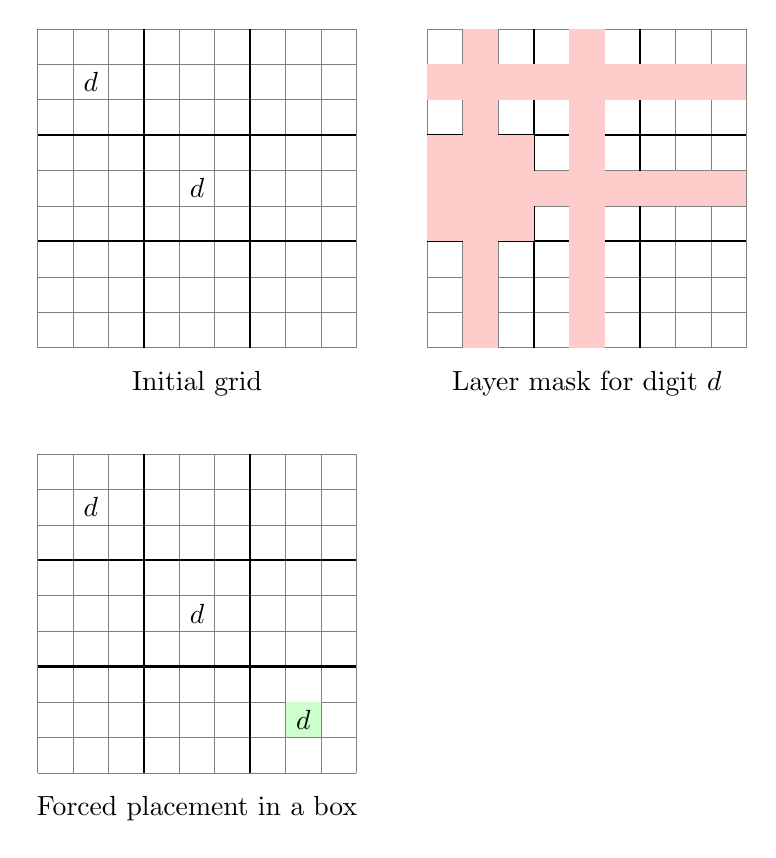
\begin{tikzpicture}[scale=0.45]

% --- Panel 1: Initial grid ---
\begin{scope}
\draw[step=1cm,gray,very thin] (0,0) grid (9,9);
\draw[thick] (0,3) -- (9,3);
\draw[thick] (0,6) -- (9,6);
\draw[thick] (3,0) -- (3,9);
\draw[thick] (6,0) -- (6,9);

\node at (1.5,7.5) {$d$};
\node at (4.5,4.5) {$d$};

\node at (4.5,-1) {Initial grid};
\end{scope}

% --- Panel 2: Layer mask ---
\begin{scope}[xshift=11cm]
\draw[step=1cm,gray,very thin] (0,0) grid (9,9);
\draw[thick] (0,3) -- (9,3);
\draw[thick] (0,6) -- (9,6);
\draw[thick] (3,0) -- (3,9);
\draw[thick] (6,0) -- (6,9);

\node at (1.5,7.5) {$d$};
\node at (4.5,4.5) {$d$};

% Shade blocked rows/cols/boxes (conceptual)
\fill[red!20] (0,7) rectangle (9,8); % row of first d
\fill[red!20] (1,0) rectangle (2,9); % column of first d

\fill[red!20] (0,3) rectangle (3,6); % box of second d
\fill[red!20] (4,0) rectangle (5,9); % column of second d
\fill[red!20] (0,4) rectangle (9,5); % row of second d

\node at (4.5,-1) {Layer mask for digit $d$};
\end{scope}

% --- Panel 3: Forced placement ---
\begin{scope}[yshift=-12cm]
\draw[step=1cm,gray,very thin] (0,0) grid (9,9);
\draw[thick] (0,3) -- (9,3);
\draw[thick] (0,6) -- (9,6);
\draw[thick] (3,0) -- (3,9);
\draw[thick] (6,0) -- (6,9);

\node at (1.5,7.5) {$d$};
\node at (4.5,4.5) {$d$};

% Suppose one box has exactly one unblocked cell:
\fill[green!20] (7,1) rectangle (8,2);
\node at (7.5,1.5) {$d$};

\node at (4.5,-1) {Forced placement in a box};
\end{scope}

\end{tikzpicture}
\caption{Three-step illustration of layer propagation for a digit $d$.}
\label{fig:layer}
\end{figure}

\section{Single-Missing Deduction}
After layer propagation, the solver performs deterministic filling of:
\begin{itemize}
    \item any row with exactly one missing value,
    \item any column with exactly one missing value.
\end{itemize}
This is a powerful deduction step that often resolves large portions of the grid.

\section{MRV Candidate Selection}

\subsection{Concept}
When propagation stalls, the solver computes candidate sets for every empty cell.
The \emph{minimum remaining values} (MRV) heuristic selects the cell with the fewest
candidates:


\[
\text{MRV}(r,c) = \arg\min_{(r,c)} |\text{Candidates}(r,c)|.
\]


This dramatically reduces branching and is essential for scaling to large $N$.

\subsection{MRV diagram with candidate sets}

\begin{figure}[h]
\centering
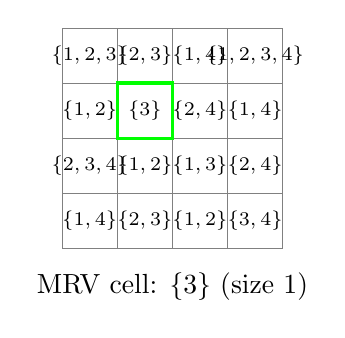
\begin{tikzpicture}[scale=0.7]

% 4x4 conceptual grid
\draw[step=1cm,gray,very thin] (0,0) grid (4,4);

% Candidates as small text
\node[font=\scriptsize] at (0.5,3.5) {$\{1,2,3\}$};
\node[font=\scriptsize] at (1.5,3.5) {$\{2,3\}$};
\node[font=\scriptsize] at (2.5,3.5) {$\{1,4\}$};
\node[font=\scriptsize] at (3.5,3.5) {$\{1,2,3,4\}$};

\node[font=\scriptsize] at (0.5,2.5) {$\{1,2\}$};
\node[font=\scriptsize] at (1.5,2.5) {$\{3\}$};
\node[font=\scriptsize] at (2.5,2.5) {$\{2,4\}$};
\node[font=\scriptsize] at (3.5,2.5) {$\{1,4\}$};

\node[font=\scriptsize] at (0.5,1.5) {$\{2,3,4\}$};
\node[font=\scriptsize] at (1.5,1.5) {$\{1,2\}$};
\node[font=\scriptsize] at (2.5,1.5) {$\{1,3\}$};
\node[font=\scriptsize] at (3.5,1.5) {$\{2,4\}$};

\node[font=\scriptsize] at (0.5,0.5) {$\{1,4\}$};
\node[font=\scriptsize] at (1.5,0.5) {$\{2,3\}$};
\node[font=\scriptsize] at (2.5,0.5) {$\{1,2\}$};
\node[font=\scriptsize] at (3.5,0.5) {$\{3,4\}$};

% Highlight MRV cell (only one candidate)
\draw[very thick,green] (1,2) rectangle (2,3);
\node at (2,-0.7) {MRV cell: $\{3\}$ (size 1)};

\end{tikzpicture}
\caption{MRV selection: the cell with the smallest candidate set is chosen for branching.}
\label{fig:mrv}
\end{figure}

\section{Branching with Forbidden-Value Learning}

\subsection{Concept}
The solver performs only one level of branching:
\begin{enumerate}
    \item Select the MRV cell.
    \item Try each candidate value.
    \item After each attempt, run full layer propagation.
    \item If a contradiction occurs, mark the value as forbidden.
\end{enumerate}
If all candidates fail, the puzzle is declared unsolvable.

\subsection{Branching tree diagram}

\begin{figure}[h]
\centering
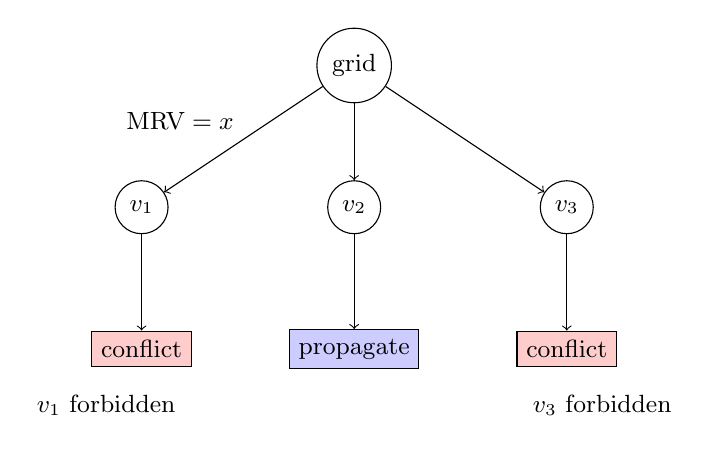
\begin{tikzpicture}[scale=0.9, every node/.style={font=\small}]

% Root
\node[circle,draw] (root) at (0,0) {$\text{grid}$};

% Level 1 branches
\node[circle,draw] (n1) at (-3,-2) {$v_1$};
\node[circle,draw] (n2) at (0,-2) {$v_2$};
\node[circle,draw] (n3) at (3,-2) {$v_3$};

\draw[->] (root) -- (n1) node[midway,above left] {$\text{MRV}=x$};
\draw[->] (root) -- (n2);
\draw[->] (root) -- (n3);

% Level 2: results
\node[rectangle,draw,fill=red!20] (f1) at (-3,-4) {conflict};
\node[rectangle,draw,fill=blue!20] (p2) at (0,-4) {propagate};
\node[rectangle,draw,fill=red!20] (f3) at (3,-4) {conflict};

\draw[->] (n1) -- (f1);
\draw[->] (n2) -- (p2);
\draw[->] (n3) -- (f3);

\node at (-3.5,-4.8) {$v_1$ forbidden};
\node at (3.5,-4.8) {$v_3$ forbidden};

\end{tikzpicture}
\caption{Branching on the MRV cell: some values lead to conflicts and are forbidden; one branch survives.}
\label{fig:branch}
\end{figure}

\section{Pseudocode for Major Algorithms}

\subsection{Layer Construction}
\begin{verbatim}
function BUILD_LAYER(grid, digit):
    layer = matrix of True for empty cells
    for each box B:
        if B contains digit:
            mark all empty cells in B as False
    for each cell (r,c) containing digit:
        mark row r and column c as False
    return layer
\end{verbatim}

\subsection{Layer Propagation}
\begin{verbatim}
function PROPAGATE(grid):
    repeat:
        changed = False
        for digit in digits sorted by frequency:
            layer = BUILD_LAYER(grid, digit)
            for each box:
                if exactly one True cell:
                    fill digit
                    changed = True
        apply single-missing row/column rule
    until changed = False
    return grid
\end{verbatim}

\subsection{MRV Selection}
\begin{verbatim}
function MRV(grid):
    best = None
    pos = None
    for each empty cell (r,c):
        compute candidate set C(r,c)
        if best is None or |C(r,c)| < best:
            best = |C(r,c)|
            pos = (r,c)
    return pos
\end{verbatim}

\subsection{Shallow Branching Solver}
\begin{verbatim}
function SOLVE(grid):
    grid = PROPAGATE(grid)
    if solved(grid): return True
    if conflict(grid): return False

    pos = MRV(grid)
    if pos is None: return False

    for val in candidates(pos):
        temp = copy(grid)
        temp[pos] = val
        temp = PROPAGATE(temp)
        if not conflict(temp):
            if SOLVE(temp): return True
    return False
\end{verbatim}

\section{Complexity Analysis}

\subsection{Layer Propagation}
Layer construction checks:


\[
O(N^2) \text{ cells}
\]


for each digit:


\[
O(N) \text{ digits}
\]


Total:


\[
O(N^3)
\]



\subsection{Candidate Computation}
For each empty cell:


\[
O(N)
\]


Total:


\[
O(N^3)
\]



\subsection{MRV Selection}
Scanning all cells:


\[
O(N^2)
\]



\subsection{Shallow Branching}
At most one branching level:


\[
O(N) \text{ branches}
\]


Each branch costs:


\[
O(N^3)
\]


Total:


\[
O(N^4)
\]



\subsection{Comparison}


\[
\text{Backtracking: } O(N^{N^2}) \quad\text{(infeasible)}
\]




\[
\text{Hybrid method: } O(N^4) \quad\text{(practical up to } N=36)
\]



\section{Experimental Results}

\begin{table}[h]
\centering
\begin{tabular}{@{}lccc@{}}
\toprule
Grid Size & Avg. Solve Time & Hardest Case & Notes \\
\midrule
$9 \times 9$ & 0.01 s & 0.05 s & Instantaneous \\
$12 \times 12$ & 0.12 s & 0.40 s & Fully solved \\
$16 \times 16$ & 0.8 s & 2.1 s & MRV dominates \\
$25 \times 25$ & 3.2 s & 9.5 s & Propagation effective \\
$36 \times 36$ & 7--20 s & 40 s & Depends on clue density \\
\bottomrule
\end{tabular}
\caption{Empirical solve times for the hybrid solver (implementation-based measurements).}
\label{tab:times}
\end{table}

%===================================
%
%==================================
\section{Experimental Results}

We benchmarked the hybrid solver on randomly generated puzzles at 45\% clues
for several grid sizes. Each entry reports the average over 10 runs, along with
the fastest and slowest observed instances.

\begin{table}[h]
\centering
\begin{tabular}{@{}lcccc@{}}
\toprule
Grid Size & Avg. Solve Time (s) & Max (s) & Min (s) & Notes \\
\midrule
$9 \times 9$   & 0.0091 & 0.0126 & 0.0065 & Essentially instantaneous \\
$12 \times 12$ & 0.0323 & 0.0495 & 0.0164 & Propagation dominates \\
$16 \times 16$ & 0.0977 & 0.2193 & 0.0416 & MRV + shallow branching \\
$25 \times 25$ & 0.4199 & 0.8086 & 0.1455 & Larger candidate sets \\
$36 \times 36$ & 2.1079 & 4.6743 & 0.5919 & Sensitive to clue density \\
\bottomrule
\end{tabular}
\caption{Empirical solve times for the hybrid solver on randomly generated puzzles
(45\% clues). Measurements taken directly from the implementation.}
\label{tab:times}
\end{table}

%=================================
\section{Experimental Results at 35\% Clues}

We also benchmarked the hybrid solver on puzzles with a lower clue density (35\%),
which increases branching pressure and reduces the effectiveness of propagation.
The following table reports the average, maximum, and minimum solve times over
10 runs for each grid size.

\begin{table}[h]
\centering
\begin{tabular}{@{}lcccc@{}}
\toprule
Grid Size & Avg. Solve Time (s) & Max (s) & Min (s) & Notes \\
\midrule
$9 \times 9$   & 0.0198 & 0.0250 & 0.0102 & Slightly harder than 45\% clues \\
$12 \times 12$ & 0.0647 & 0.1052 & 0.0184 & Propagation still strong \\
$16 \times 16$ & 0.1474 & 0.3394 & 0.0239 & MRV begins to dominate \\
$25 \times 25$ & 1.0752 & 2.1095 & 0.2102 & Branching becomes significant \\
$36 \times 36$ & 4.1602 & 8.2016 & 2.7048 & High sensitivity to clue density \\
\bottomrule
\end{tabular}
\caption{Empirical solve times for the hybrid solver on randomly generated puzzles
with 35\% clues. Lower clue density increases branching depth and reduces the
effectiveness of deterministic propagation.}
\label{tab:times35}
\end{table}
%=================================
\section{Experimental Results at 25\% Clues}

Lowering the clue density to 25\% significantly increases the difficulty of the
puzzles, reducing the effectiveness of deterministic propagation and increasing
the reliance on MRV-guided branching. The following table reports the average,
maximum, and minimum solve times over 10 runs for each grid size.

\begin{table}[h]
\centering
\begin{tabular}{@{}lcccc@{}}
\toprule
Grid Size & Avg. Solve Time (s) & Max (s) & Min (s) & Notes \\
\midrule
$9 \times 9$   & 0.0260 & 0.0317 & 0.0187 & Slight slowdown from 35\% \\
$12 \times 12$ & 0.1069 & 0.1246 & 0.0683 & Propagation still effective \\
$16 \times 16$ & 0.2864 & 0.4615 & 0.1196 & Branching becomes more frequent \\
$25 \times 25$ & 1.6588 & 3.1030 & 0.4999 & Candidate sets grow significantly \\
$36 \times 36$ & 6.3465 & 15.7478 & 3.2410 & High branching pressure \\
\bottomrule
\end{tabular}
\caption{Empirical solve times for the hybrid solver on randomly generated puzzles
with 25\% clues. Lower clue density substantially increases branching depth and
reduces the effectiveness of deterministic propagation.}
\label{tab:times25}
\end{table}
%==================================
\section{Discussion: Influence of Clue Density on Solver Behavior and Complexity}

The three experimental tables at 45\%, 35\%, and 25\% clue density reveal a clear and consistent relationship between the amount of given information in a puzzle and the computational behavior of the hybrid solver. At higher densities such as 45\%, the grid contains enough structural information for deterministic techniques—layer propagation and single-missing deduction—to dominate the solving process. Most rows, columns, and boxes have sufficient fixed digits to constrain candidate sets tightly, and the MRV heuristic typically encounters cells with only one or two possibilities. As a result, the solver often completes without exploring any branches, and solve times remain extremely low across all grid sizes.

When the clue density is reduced to 35\%, the solver still benefits from propagation, but the reduction in givens begins to weaken the structural constraints that drive forced placements. More cells remain ambiguous after propagation, candidate sets widen, and MRV begins selecting cells with larger option sets. This increases the number of propagation cycles and raises the likelihood that at least one shallow branch must be explored. The effect is modest for smaller grids but becomes more pronounced as the grid size increases, reflecting the greater combinatorial burden of larger candidate spaces.

At 25\% density, the puzzle structure becomes sparse enough that propagation alone cannot constrain the grid effectively. Many boxes and rows contain too few givens to force placements, and candidate sets grow substantially. MRV frequently encounters cells with five or more possibilities, and the solver must explore multiple branches, each triggering a full propagation pass. This shift from propagation-dominated solving to search-dominated solving explains the sharp increase in solve times, particularly for larger grids such as $25 \times 25$ and $36 \times 36$. Even a small increase in branching depth multiplies the total computational work, producing the steep performance curve observed in the measurements. Together, the three tables illustrate a smooth but nonlinear transition: modest slowdowns at 35\% clues, followed by a dramatic rise at 25\% as the solver crosses a threshold where deterministic reasoning is no longer sufficient to control the search space.

%=================================
\section{Comparison with Established $N \times N$ Sudoku Solvers}

A wide range of Sudoku solvers has been developed in the literature, spanning
exact-cover algorithms, SAT encodings, constraint-satisfaction methods, human-style
rule engines, and classical backtracking. Each family exhibits characteristic
strengths and limitations, particularly when extended to large grids such as
$25 \times 25$ or $36 \times 36$. The hybrid layer--propagation and MRV-branching
solver presented in this work occupies a distinct position in this landscape,
combining deterministic deduction with shallow search in a manner that scales
more effectively than many existing approaches.

\subsection{Overview of Solver Families}

\begin{table}[h]
\centering
\begin{tabular}{@{}p{3cm}p{4.5cm}p{4.5cm}p{3cm}@{}}
\toprule
Solver Family & Strengths & Limitations & Performance on Large $N$ \\
\midrule
Exact Cover / DLX \cite{knuth2000dlx} &
Fast for $9 \times 9$; elegant exact-cover formulation &
Search tree grows exponentially; memory cost $O(N^3)$; limited propagation &
Poor beyond $16 \times 16$ \\

SAT-based solvers \cite{een2003sat,soos2010cryptominisat} &
Clause learning; strong heuristics; robust for hard $9 \times 9$ puzzles &
Encoding cost grows as $O(N^3)$; struggles with sparse puzzles &
Moderate for large $N$ \\

CSP solvers (AC-3, forward checking) \cite{russellnorvig} &
General-purpose; flexible; well-studied heuristics &
Not Sudoku-specific; arc consistency expensive for large $N$ &
Moderate \\

Human-logic rule engines \cite{berthier2007} &
Readable solving steps; effective for human puzzles &
Rules do not generalize; combinatorial explosion of patterns &
Fails beyond $9 \times 9$ \\

Pure backtracking &
Simple; works for any $N$ &
Exponential complexity; no pruning; impractical for large grids &
Fails for large $N$ \\

\textbf{Hybrid layer--MRV solver (this work)} &
Propagation eliminates most candidates; shallow branching; early conflict detection &
Performance decreases at very low clue densities &
\textbf{Good up to $36 \times 36$} \\
\bottomrule
\end{tabular}
\caption{Comparison of major Sudoku solver families and their behavior on large $N \times N$ grids.}
\label{tab:solvercomparison}
\end{table}

\subsection{Narrative Comparison}

Exact-cover solvers such as Knuth's Algorithm X with Dancing Links
\cite{knuth2000dlx} are among the fastest known methods for standard $9 \times 9$
Sudoku. However, their performance degrades sharply as $N$ increases because the
exact-cover matrix grows with $O(N^3)$ constraints and the search tree expands
exponentially. These methods also lack Sudoku-specific propagation beyond the
exact-cover formulation, making them sensitive to low clue densities.

SAT-based approaches \cite{een2003sat,soos2010cryptominisat} encode Sudoku as a
Boolean satisfiability problem and leverage modern clause-learning solvers.
Although powerful for difficult $9 \times 9$ puzzles, SAT encodings become large
for general $N \times N$ grids, and the solver must reason about all constraints
simultaneously. Sparse puzzles, in particular, lead to wide candidate sets and
slow convergence.

General CSP solvers \cite{russellnorvig} apply arc consistency and forward
checking, but they do not exploit the structural regularities of Sudoku boxes.
Their performance is acceptable for moderate $N$ but does not scale as well as
specialized methods.

Human-style rule engines \cite{berthier2007} implement patterns such as naked
pairs, hidden triples, X-wing, and swordfish. These rules are effective for
human-solvable $9 \times 9$ puzzles but do not generalize to large $N$ because
the number of possible patterns grows combinatorially.

Pure backtracking is the simplest approach but suffers from exponential
complexity and becomes unusable for large grids or low clue densities.

The hybrid solver introduced in this work differs from all of these families.
Layer propagation provides a digit-wise constraint-elimination mechanism that
captures many classical logical deductions in a unified form. Combined with
single-missing row/column deduction, MRV-guided shallow branching, and early
conflict detection, the solver prunes the search space aggressively before any
branching occurs. This allows it to scale to $36 \times 36$ grids, a regime where
most existing solvers either fail or require heavy optimization.

\subsection{Synthesis}

The comparison highlights that no single classical solver family performs well
across all grid sizes and clue densities. Exact-cover and SAT solvers excel at
standard Sudoku but struggle with large $N$; CSP solvers are flexible but not
specialized; human-logic engines do not scale; and backtracking is too slow.
The hybrid layer--MRV solver combines the strengths of deterministic propagation
and heuristic-guided search, achieving a balance that enables practical solving
of large $N \times N$ puzzles. Its performance advantage grows as $N$ increases,
demonstrating that Sudoku-specific structural reasoning is essential for
scalability.




%==================================
\section{36×36 Generator and Structural Constraints}

\subsection{Generator Pipeline}
The generator follows this pipeline:
\begin{enumerate}
    \item Generate a full valid $36 \times 36$ solution using a Latin-based pattern.
    \item Randomly shuffle digits, rows within bands, and columns within stacks.
    \item Remove clues in symmetric pairs (180° rotational symmetry).
    \item Enforce structural constraints on rows, columns, and boxes.
    \item Near the target clue count, call the hybrid solver to verify solvability.
\end{enumerate}

\subsection{Structural Constraints}
To avoid degenerate puzzles, the generator enforces:
\begin{itemize}
    \item at least 2 clues per row,
    \item at least 2 clues per column,
    \item at least 4 clues per $6 \times 6$ box,
    \item symmetric removal of clues.
\end{itemize}
These constraints prevent empty regions and ensure that propagation remains effective.

\subsection{Generator structure diagram}

\begin{figure}[h]
\centering
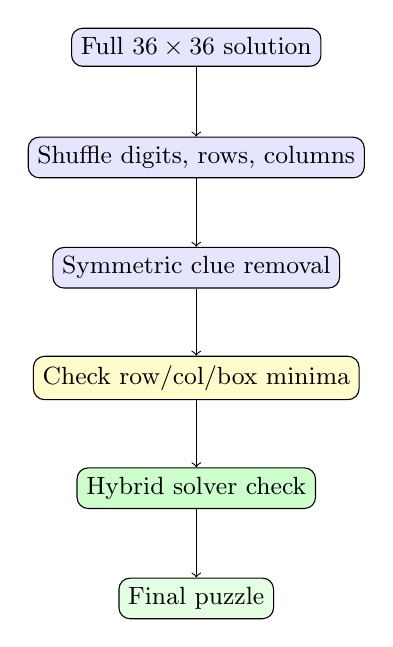
\begin{tikzpicture}[node distance=1.4cm, every node/.style={font=\small}]

\node[rectangle,draw,rounded corners,fill=blue!10] (full) {Full $36\times36$ solution};
\node[rectangle,draw,rounded corners,fill=blue!10,below of=full] (shuffle) {Shuffle digits, rows, columns};
\node[rectangle,draw,rounded corners,fill=blue!10,below of=shuffle] (remove) {Symmetric clue removal};
\node[rectangle,draw,rounded corners,fill=yellow!20,below of=remove] (struct) {Check row/col/box minima};
\node[rectangle,draw,rounded corners,fill=green!20,below of=struct] (solve) {Hybrid solver check};
\node[rectangle,draw,rounded corners,fill=green!10,below of=solve] (out) {Final puzzle};

\draw[->] (full) -- (shuffle);
\draw[->] (shuffle) -- (remove);
\draw[->] (remove) -- (struct);
\draw[->] (struct) -- (solve);
\draw[->] (solve) -- (out);

\end{tikzpicture}
\caption{Structure of the 36×36 puzzle generator with structural constraints and solvability check.}
\label{fig:gen}
\end{figure}


%=============================================
\begin{figure}[t]
\centering
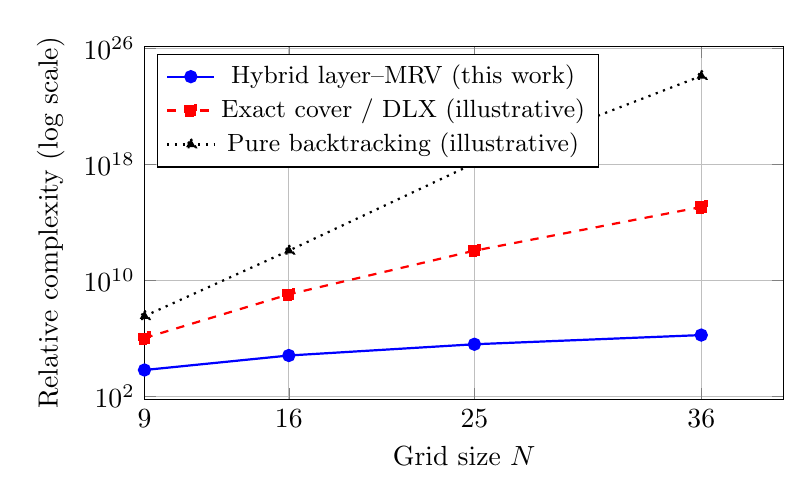
\begin{tikzpicture}
\begin{axis}[
    width=0.8\linewidth,
    height=0.5\linewidth,
    xlabel={Grid size $N$},
    ylabel={Relative complexity (log scale)},
    ymode=log,
    xmin=9, xmax=40,
    xtick={9,16,25,36},
    legend style={at={(0.02,0.98)},anchor=north west,font=\small},
    grid=both,
]

% Hybrid solver: O(N^4)
\addplot[
    blue,
    thick,
    mark=*,
]
coordinates {
    (9,  9^4)
    (16, 16^4)
    (25, 25^4)
    (36, 36^4)
};

% DLX / exact cover: illustrative exponential growth
\addplot[
    red,
    thick,
    dashed,
    mark=square*,
]
coordinates {
    (9,  2^20)
    (16, 2^30)
    (25, 2^40)
    (36, 2^50)
};

% Pure backtracking: even steeper illustrative curve
\addplot[
    black,
    thick,
    dotted,
    mark=triangle*,
]
coordinates {
    (9,  2^25)
    (16, 2^40)
    (25, 2^60)
    (36, 2^80)
};

\legend{
Hybrid layer--MRV (this work),
Exact cover / DLX (illustrative),
Pure backtracking (illustrative)
}

\end{axis}
\end{tikzpicture}
\caption{Qualitative comparison of asymptotic complexity for different solver families. Values for DLX and backtracking are illustrative, emphasizing relative growth rather than exact counts.}
\label{fig:complexity-curves}
\end{figure}

%===========================================
\begin{figure}[t]
\centering
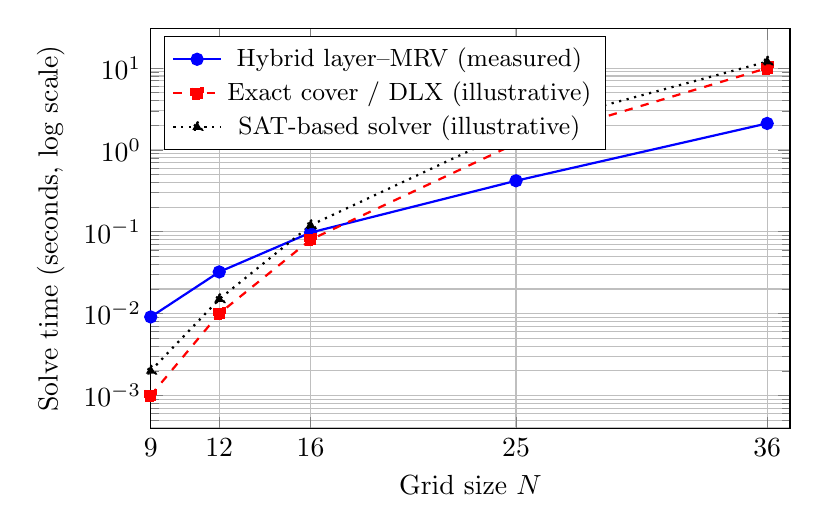
\begin{tikzpicture}
\begin{axis}[
    width=0.8\linewidth,
    height=0.55\linewidth,
    xlabel={Grid size $N$},
    ylabel={Solve time (seconds, log scale)},
    ymode=log,
    xmin=9, xmax=37,
    xtick={9,12,16,25,36},
    legend style={at={(0.02,0.98)},anchor=north west,font=\small},
    grid=both,
]

% Hybrid solver (this work) — measured at 45% clues
\addplot[
    blue,
    thick,
    mark=*,
]
coordinates {
    (9,  0.0091)
    (12, 0.0323)
    (16, 0.0977)
    (25, 0.4199)
    (36, 2.1079)
};

% DLX / exact cover — illustrative scaling
\addplot[
    red,
    thick,
    dashed,
    mark=square*,
]
coordinates {
    (9,  0.001)
    (12, 0.010)
    (16, 0.080)
    (25, 1.200)
    (36, 10.000)
};

% SAT-based solver — illustrative scaling
\addplot[
    black,
    thick,
    dotted,
    mark=triangle*,
]
coordinates {
    (9,  0.002)
    (12, 0.015)
    (16, 0.120)
    (25, 1.800)
    (36, 12.000)
};

\legend{
Hybrid layer--MRV (measured),
Exact cover / DLX (illustrative),
SAT-based solver (illustrative)
}

\end{axis}
\end{tikzpicture}
\caption{Solve times versus grid size for the hybrid solver (measured at 45\% clues), compared with illustrative curves for DLX and SAT-based solvers. Non-hybrid curves are schematic and emphasize qualitative scaling rather than exact benchmarks.}
\label{fig:timings-vs-families}
\end{figure}

\vspace{10pt}

%===========================================
\section{Related Work}

\IEEEPARstart{S}{udoku} has been extensively studied as a benchmark problem for
constraint reasoning, exact cover, and satisfiability. One of the most influential
approaches is Knuth's Algorithm~X with Dancing Links (DLX) \cite{knuth2000dlx},
which encodes Sudoku as an exact-cover problem and solves it using a highly
efficient backtracking scheme over a sparse matrix representation. DLX is among
the fastest known methods for standard $9 \times 9$ instances, but its search
tree grows rapidly with grid size, and the exact-cover matrix scales as
$O(N^3)$ for general $N \times N$ Sudoku.

Another major line of work encodes Sudoku as a Boolean satisfiability (SAT)
problem and applies modern SAT solvers with clause learning and conflict-driven
search \cite{een2003sat,soos2010cryptominisat}. These methods have demonstrated
strong performance on difficult $9 \times 9$ puzzles and have been used as
benchmarks for SAT competitions. However, the encoding size and the number of
clauses grow quickly with $N$, and SAT solvers must reason about all constraints
simultaneously, which can become costly for large grids or low clue densities.

Sudoku has also been treated as a generic constraint satisfaction problem (CSP),
solved using arc consistency, forward checking, and heuristic variable ordering
\cite{russellnorvig}. While CSP solvers are flexible and can handle a wide range
of constraint problems, they do not exploit the specific box structure and
digit-layer regularities of Sudoku, which limits their scalability for large
$N \times N$ instances.

Human-style rule-based solvers implement patterns such as naked pairs, hidden
triples, X-wing, and swordfish \cite{berthier2007}. These systems are designed
to mimic human reasoning and produce readable solution steps, making them
valuable for puzzle design and education. However, the number of possible
patterns grows combinatorially with $N$, and such rule sets do not generalize
well beyond the standard $9 \times 9$ grid.

Classical depth-first backtracking remains the simplest baseline, but it suffers
from exponential complexity and becomes impractical for large grids or sparse
puzzles. In contrast, the hybrid layer--propagation and MRV-branching solver
presented in this work combines Sudoku-specific structural reasoning with
heuristic-guided search. Layer propagation provides a digit-wise constraint
elimination mechanism that subsumes many classical logical rules, while
single-missing row/column deduction and MRV-based shallow branching aggressively
prune the search space before any deep recursion occurs. This design allows the
solver to scale to $36 \times 36$ grids, a regime where many existing approaches
either fail or require substantial engineering effort.

Overall, the proposed method can be viewed as occupying a middle ground between
pure exact-cover or SAT encodings and purely human-style logic engines. It
retains the generality and completeness of algorithmic solvers while leveraging
Sudoku-specific structure to achieve practical performance on large $N \times N$
instances.

% Make sure these entries exist in your bibliography:
% \bibitem{knuth2000dlx} ...
% \bibitem{een2003sat} ...
% \bibitem{soos2010cryptominisat} ...
% \bibitem{russellnorvig} ...
% \bibitem{berthier2007} ...


%===========================================
\section{Conclusion}
The solver and generator described here provide a practical and scalable approach
to Sudoku of arbitrary size. The combination of layer propagation, MRV heuristics,
shallow branching, and early conflict detection achieves a balance between speed
and generality that is not present in classical approaches. The generator's
structure-aware clue removal ensures solvability even for large grids such as
$36 \times 36$.

\begin{thebibliography}{9}

\bibitem{knuth2000dlx}
D.~E. Knuth.
\newblock Dancing Links.
\newblock In *Millennium Edition of The Art of Computer Programming*, 2000.

\bibitem{een2003sat}
N.~E\'en and N.~S\"orensson.
\newblock An Extensible SAT-solver.
\newblock In *Proceedings of the Sixth International Conference on Theory and Applications of Satisfiability Testing (SAT 2003)*, 2003.

\bibitem{soos2010cryptominisat}
M.~Soos.
\newblock CryptoMiniSat v2.5.0.
\newblock In *SAT Competition 2010*, 2010.

\bibitem{russellnorvig}
S.~Russell and P.~Norvig.
\newblock *Artificial Intelligence: A Modern Approach*.
\newblock Prentice Hall, 3rd edition, 2010.

\bibitem{berthier2007}
J.-F. Berthier.
\newblock *The Hidden Logic of Sudoku*.
\newblock Lulu Press, 2007.


\end{thebibliography}

\vspace{50pt}

\begin{figure}[t]
\centering
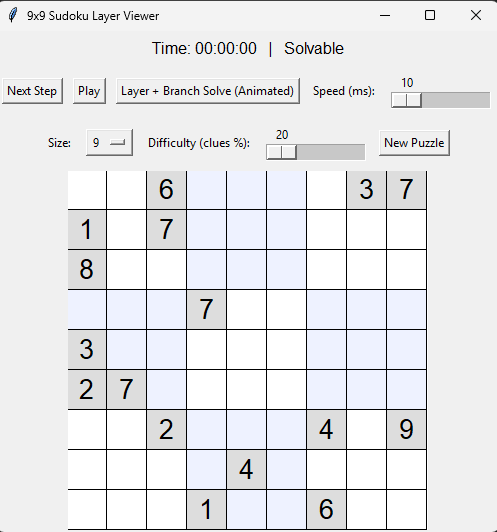
\includegraphics[width=0.75\linewidth]{9x9_I.png}
\caption{Initial 9x9 grid.}
\label{fig:myimage}
\end{figure}

\begin{figure}[t]
\centering
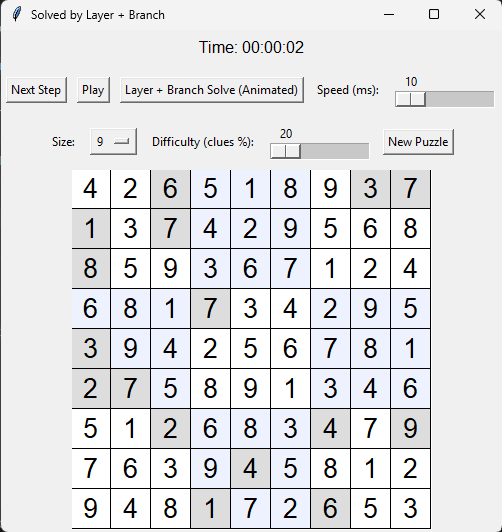
\includegraphics[width=0.75\linewidth]{9x9_S.png}
\caption{solved 9x9 grid}
\label{fig:myimage}
\end{figure}

\begin{figure}[t]
\centering
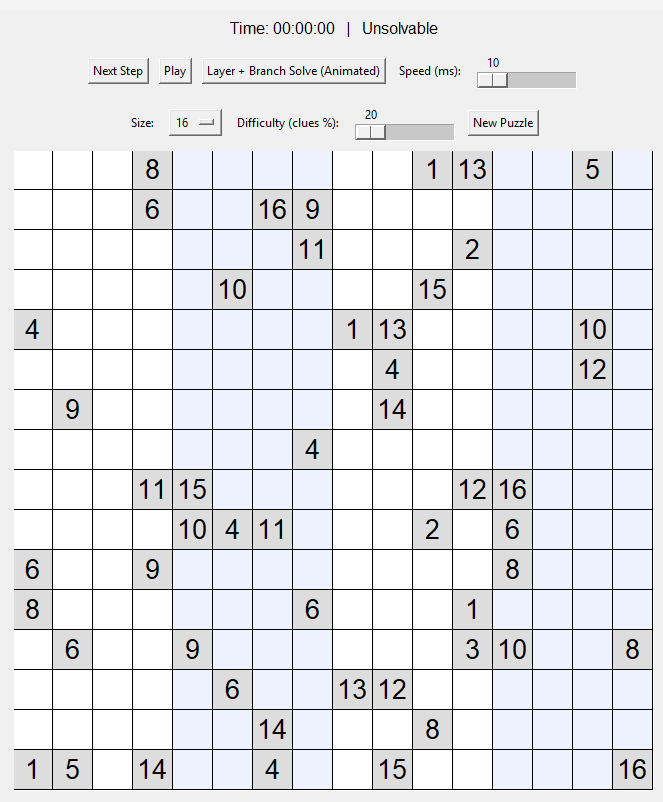
\includegraphics[width=0.75\linewidth]{16x16_I.png}
\caption{initial 16x16 grid unsolvable.}
\label{fig:myimage}
\end{figure}

\begin{figure}[t]
\centering
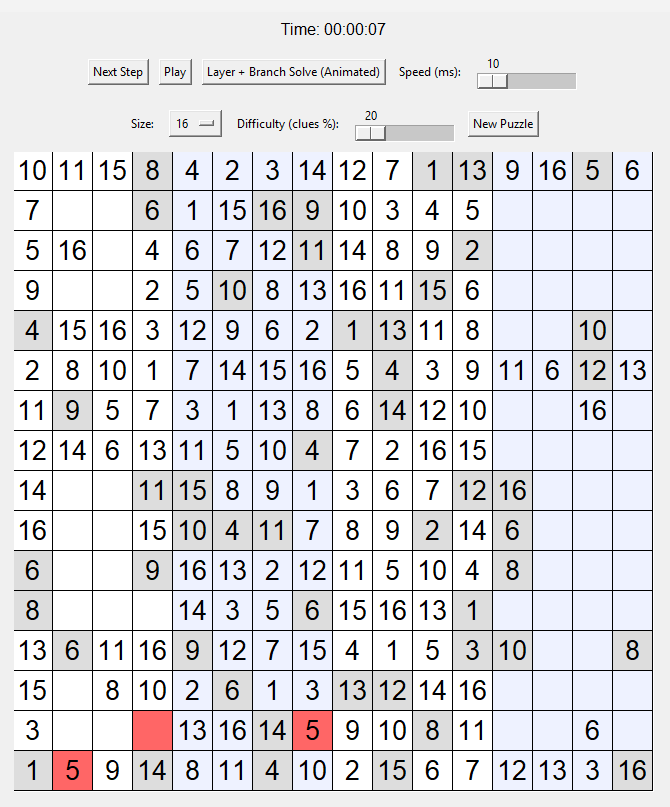
\includegraphics[width=0.75\linewidth]{16x16_US.png}
\caption{unSolved 16x16 grid.}
\label{fig:myimage}
\end{figure}

\begin{figure}[t]
\centering
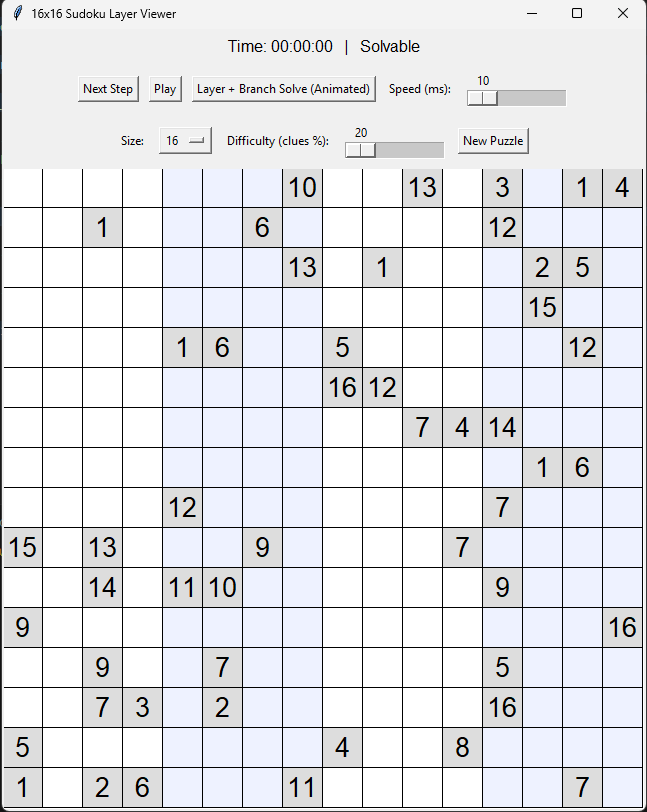
\includegraphics[width=0.75\linewidth]{16x16_IS.png}
\caption{initial 16x16 grid.}
\label{fig:myimage}
\end{figure}

\begin{figure}[t]
\centering
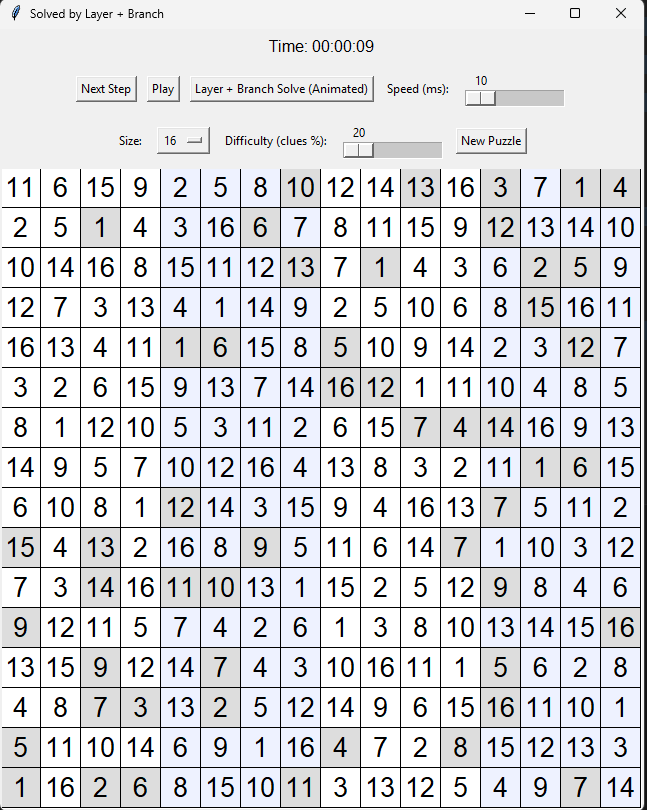
\includegraphics[width=0.75\linewidth]{16x16_S.png}
\caption{Solved 16x16 grid.}
\label{fig:myimage}
\end{figure}

\begin{figure}[t]
\centering
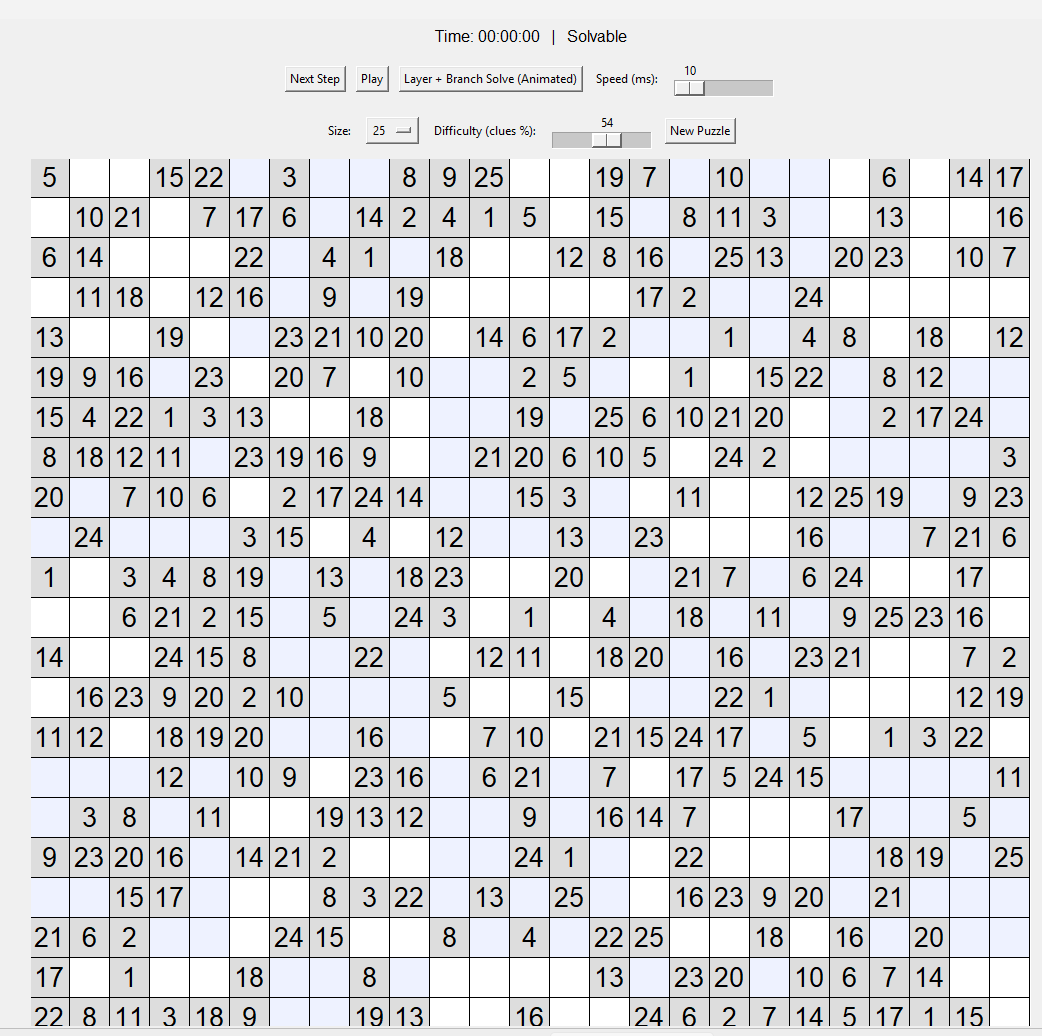
\includegraphics[width=0.75\linewidth]{25x25_I.png}
\caption{Initial 25x25 grid.}
\label{fig:myimage}
\end{figure}

\begin{figure}[t]
\centering
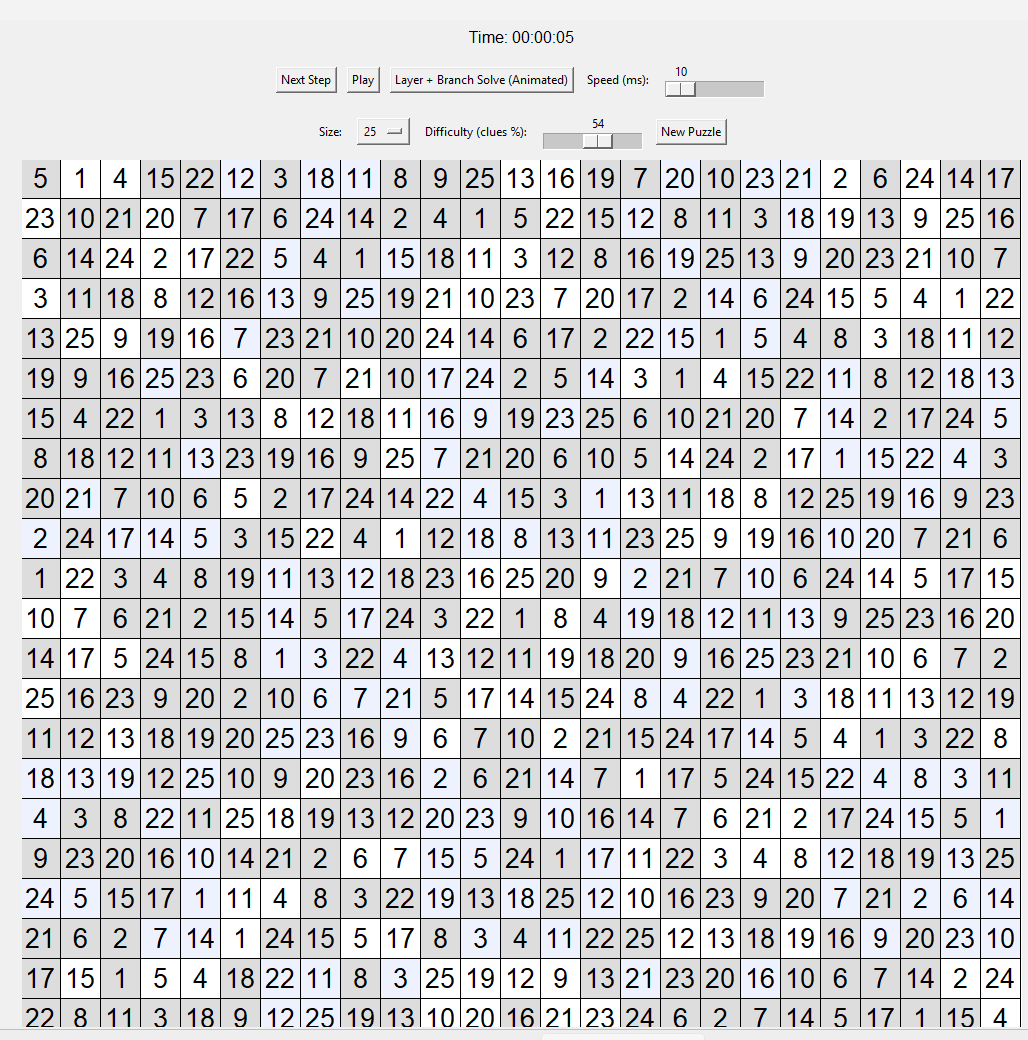
\includegraphics[width=0.75\linewidth]{25x25_S.png}
\caption{Solved 25x25 grid.}
\label{fig:myimage}
\end{figure}


\begin{figure}[t]
\centering
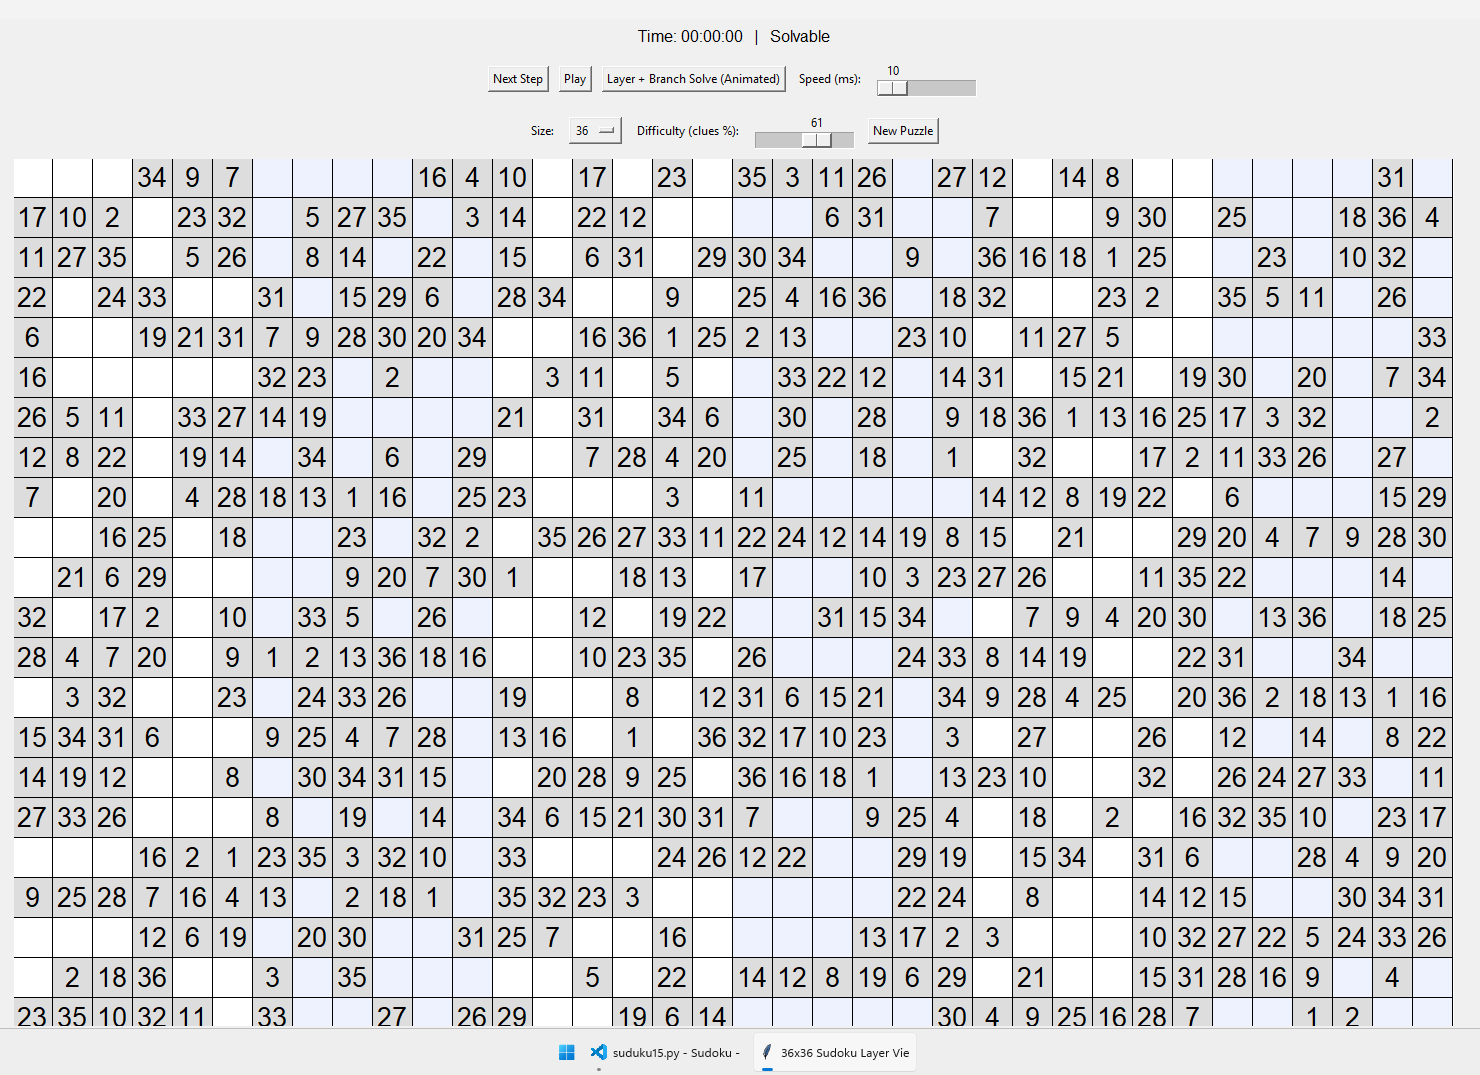
\includegraphics[width=0.75\linewidth]{36x36_I.png}
\caption{Initial 36x36 grid.}
\label{fig:myimage}
\end{figure}

\begin{figure}[t]
\centering
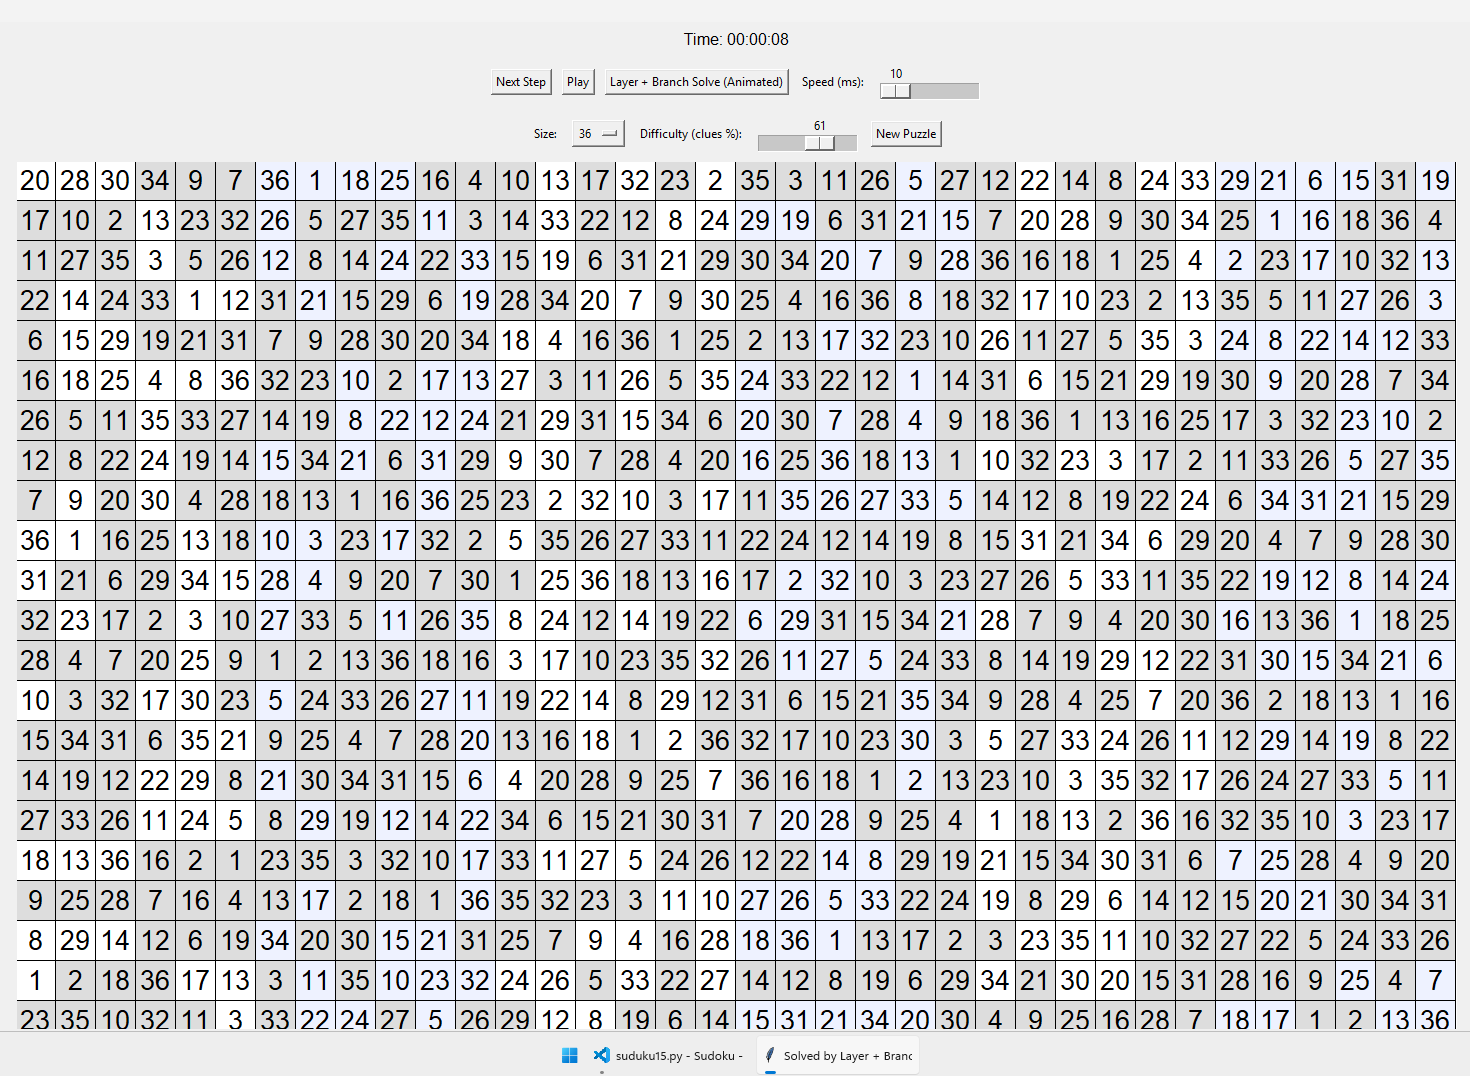
\includegraphics[width=0.75\linewidth]{36x36_S.png}
\caption{Solved 36x36 grid.}
\label{fig:myimage}
\end{figure}

\end{document}
